% elmer3-space-marching.tex
% Overall LaTeX format adapted from PJ's elmer3 user guide
% and copied here from Wilson's k-w Turbulence Guide
% 
% Fabian Zander, Mar 10 2011
%

\documentclass[12pt,a4paper]{article}
\usepackage[body={16cm,24.5cm}]{geometry}
\usepackage{pstricks}
\usepackage{graphicx}
\usepackage{listings}
\lstset{basicstyle=\scriptsize,identifierstyle=,keywordstyle=}

%------------------------------------------------------------------
% a couple horizontal bars to delimit embedded code
% the width suits the page size set above and
% the mathmode eliminates spaces between the three elements
\newcommand{\topbar}{\ensuremath{
    \rule{0.1mm}{2.0mm} \rule[2.0mm]{159.5mm}{0.1mm} \rule{0.1mm}{2.0mm}
}}
\newcommand{\bottombar}{\ensuremath{
    \rule{0.1mm}{2.0mm} \rule{159.5mm}{0.1mm} \rule{0.1mm}{2.0mm}
}}
\newcommand{\topbarshort}{\ensuremath{
    \rule{0.1mm}{2.0mm} \rule[2.0mm]{149.5mm}{0.1mm} \rule{0.1mm}{2.0mm}
}}
\newcommand{\bottombarshort}{\ensuremath{
    \rule{0.1mm}{2.0mm} \rule{149.5mm}{0.1mm} \rule{0.1mm}{2.0mm}
}}
%------------------------------------------------------------------

\title{
    Space Marching in Eilmer3: \\
    User guide and test cases
}
\author{
    The University of Queensland \\
    School of Mechanical \& Mining Engineering \\
    Research Report Number 2011/03 
    \vspace{0.5cm} \\
    F. Zander, 
    P. A. Jacobs\thanks{Queensland Geothermal Energy Centre of 
     Excellence, The University of Queensland, Brisbane, Australia.},
    R. J. Gollan, 
    W.Y.K. Chan and 
    R. M. Kirchhartz\\
    {Centre for Hypersonics, The University of 
     Queensland, Brisbane, Australia.}
\\
}

\usepackage{subfigure}   % Adds capability to input sub-figures

\begin{document}
\maketitle

\centerline{\textbf{Abstract}}
\medskip
This report provides a basic outline on the use of space marching in Eilmer3. Space marching offers a computationally cheap method of conducting CFD calculations of simple geometries and flows. This report details the use and some of the limitations of the space marching solver and gives two examples of the solver being used. The first example is a simple stream tube case and the second is a sample scramjet geometry. The intention of this report is that it will lead to further computational experiments with space marching, particularly for shock tunnel simulations.
\newpage
\tableofcontents

%-------------------------------------------------------------------
% introduction.tex

\newpage
\section{Introduction}
\label{chapter-introduction}
%
This report provides the basic outline on using space marching in Eilmer3. Eilmer3 is an integrated collection of programs for the simulation of transient compressible flow in two- and three-dimensions. Detailed descriptions of Eilmer3 can be found in the reports by Jacobs et al. \cite{Jacobs2008,Jacobs2010}.

The space marching solver in Eilmer3 is a subset of the time-dependent solver implemented to reduce computational time. Computational time savings of up to 85\% have been demonstrated in some test cases. This report details some specific information in regards to what can and cannot be done with space marching and provides an example of space marching in use with comparisons to the time-dependent solver (see section \ref{chapter3-axi-scramjet}).

\subsection{Solver Description}
%\label{}

The original space marching solver implemented in Eilmer3 considered each block in the domain individually and solved them sequentially with the time-dependent solver. The time computed for each block was the total simulation time divided by the number of blocks. This functioned reasonably well as a first run for any particular case however the data exchange between each of the blocks caused inaccuracies to accumulate in a downstream direction. The code has recently been updated to remove this error source by solving two blocks at a time and then moving downstream in one-block increments. This has provided a large improvement in the results as demonstrated by some of the results shown in section \ref{chapter3-axi-scramjet}.

The current space marching solver computes individual blocks using the time-dependent solver in sequence. It does this in two block increments in order to avoid block-boundary data-transfer errors. Blocks \textit{n} and \textit{n+1} are solved to time \textit{dt} (\textit{dt} is the total time divided by the number of blocks). The solver then moves forward one block and solves blocks \textit{n+1} and \textit{n+2} and continues this process until all the blocks have been solved. Each set of two blocks is considered as an independent problem where the inflow is defined by the ghost cells of the previous block and the outflow is considered an ExtrapolateOutBC() (see the user guide for a description of this boundary condition \cite{Jacobs2008}). As the solver moves along the blocks the previous ExtrapolateOutBC() is converted back to a block boundary exchange condition which is solved accurately in the next step. This process of solving across the block boundaries removes any errors that may have been introduced by the applied boundary conditions in the individual block computations. The new code that has been implemented into Eilmer3 can be found in Appendix \ref{code}.

The time dependent solver code has also been modified so that when solving individual space marching components the time step used is carried over from block to block. This is a recent modification to the code that removes a large number of computational steps compared with the old code where the time stepping was restarted for each block.

\subsection{Current Limitations}
%\label{}

When using the space marching solver, there are some limitations the user should be aware of: (a) there are limitations with regards to physical modelling; and (b) there are limitations associated with the coding implementation.

The physical modelling restriction with all space marching solvers is that the flow must travel only downstream, predominantly supersonically. This means that separation/recirculation areas and any other regions causing upstream flow must be avoided. The only exception to this is if the separation zone is small enough to be contained within a single block. As all the individual blocks are solved using the time resolved solver if the area is contained with a single block this will be modelled properly.

In terms of implementation the solver is currently limited to only one row of blocks. This means that the geometry must be sufficiently simple so that it can be modelled in this fashion with each block situated downstream of the previous block. This also means that the solver runs on a single CPU only however the `real time' taken for the computation is still significantly less than than a MPI process (depending on the number of processors used) justifying the use of this solver. These limitations could be removed at a later date if necessary.

\subsection{Recommended guidelines for using the space marching solver in Eilmer3}
%\label{}

Setting up Eilmer3 to run the space marching solver is done by configuring the \textit{sequence\_blocks} value. This is done with \newline
\centerline{\textit{gdata.sequence\_blocks $=$ 1}}
\newline
At this point the space marching is activated however the efficiency of the computation is dependent on the rest of the model being configured appropriately. 

The easiest way to set up the blocks within Eilmer3 is to use the SuperBlock construction method ( see reference \cite{Jacobs2008}). If multiple SuperBlocks are used then they can only be joined on the east-west boundaries. When specifying the divisions of SuperBlocks the \textit{nbj} value must be set to 1 and the block can be split into any number of sub-blocks in the \textit{nbi} direction. The more blocks there are the quicker the solver will reach completion however some caution must be taken not to make the blocks too thin in the flow direction. Commonly there have been 100 blocks used with 20 cells per block however the exact numbers used will also be affected by the cell spacing.

The space marching solver does not give intermediate results (unlike the time resolved solver) and therefore there is currently no real check for time-convergence. Previous experience has shown that the result is well converged after approximately 3 flow lengths (see section \ref{chapter3-axi-scramjet}) however this is something that should be considered carefully when specifying the total simulation time.

% stream-tube.tex

\newpage
\section{Stream Tube}
\label{chap2-stream-tube}
%

The first example used to show the space marching solver in use is a simple stream-tube geometry. This case was initially used to verify some of the chemistry schemes being used in Eilmer3 and also demonstrates the use of the space marching solver very nicely. This model comprised of 20000 cells and the simulation was run on a 1.86GHz desktop in 19 mins on a Barrine CPU. This is quite a reduction in wall-clock time when compared to the 2 hours 44 mins that the simulation needed on 40 Barrine CPU's for a time-dependent solution.

The inflow conditions used were taken from a Bittker and Scullin report\cite{Bittker_Scullin72} in order to check the chemistry behaviour of the code. The conditions used were: \[ u = 4500.0m/s, \quad p = 97.0kPa, \quad T = 1560.0K \] Figure \ref{fig:stream_tube_OH} shows the development of OH down the length of the stream tube which is an indicator of the combustion development.

\begin{figure}[h]
 \centering
 \includegraphics[width=0.9\linewidth]{./chap2-stream-tube/stream_tube.pdf}
 % stream_tube.pdf: 0x0 pixel, 300dpi, 0.00x0.00 cm, bb=
 \caption{OH development down the length of the tube}
 \label{fig:stream_tube_OH}
\end{figure}

\newpage
\subsection{Input script}

{\scriptsize
\begin{verbatim}
## \file hydrogen_validation.py
## \brief Eilmer3 job-spec file of a stream-tube
## \author Fabian Zander, 26th Oct 2010
##
##
## A test case to see if the hydrogen comubstion scheme is working
## This example is trying to match test case 3 from the Bittker-Scullin code 
## ( A Nasa report - NASA TN D-6586)

job_title = "Hydrogen-Air Combustion Validation"
print job_title

from math import sin, cos, pi, atan, sqrt

# Global data
gdata.dimensions = 2
gdata.title = job_title
gdata.axisymmetric_flag = 1
gdata.stringent_cfl = 1

# Gas model - thermally perfect gas - air
select_gas_model(model='thermally perfect gas', 
                 species=['O', 'O2', 'N2', 'H', 'H2', 'H2O', 'HO2', 'OH', 'H2O2'])

set_reaction_scheme("Bittker_Scullin.lua", reacting_flag=1)

gmodel = get_gas_model_ptr()

# Initial mixture taken from Bittker Scullin example on page 85 in mol fraction

mf_H2 = 0.2958
mf_O2 = 0.1480
mf_N2 = 0.5562

mf_initial = {'O':0.000, 'O2':mf_O2, 'N2':mf_N2, 'H':0.000, 'H2':mf_H2, 
	      'H2O':0.000, 'HO2':0.000, 'OH':0.000, 'H2O2':0.000}
mf = {'O':0.000, 'O2':mf_O2, 'N2':mf_N2, 'H':0.000, 'H2':mf_H2, 
      'H2O':0.000, 'HO2':0.000, 'OH':0.000, 'H2O2':0.000}

# Input inital flow conditions
# These are values taken from test case 3 in Bittker and Scullin

initial = FlowCondition(p=96.87e3, u=4551.73, v=0.0, T=1559.00, massf=gmodel.to_massf(mf_initial))
inflow = FlowCondition(p=96.87e3, u=4551.73, v=0.0, T=1559.00, massf=gmodel.to_massf(mf))

# Setting up the geometry

a = Node(0.0000, 0.0000, label="a")
b = Node(0.1000, 0.0000, label="b")
c = Node(0.1000, 0.0100, label="c")
d = Node(0.0000, 0.0100, label="d")

blk_0_north = Line(d,c)
blk_0_east = Line(b,c)
blk_0_south = Line(a,b)
blk_0_west = Line(a,d)

# Define the block, boundary conditions etc.

nx0 = 10000
ny0 = 2

patch0 = make_patch(blk_0_north, blk_0_east, blk_0_south, blk_0_west)
nbi_0 = 100
nbj_0 = 1
blk_0 = SuperBlock2D(patch0, nni=nx0, nnj=ny0, nbi=nbi_0, nbj=nbj_0,
		fill_condition=initial, label="Block-0")

print 'Block 0 has %s elements and each sub-block has %s elements' % (nx0*ny0, nx0*ny0/(nbi_0*nbj_0))

identify_block_connections()

for ib_0 in range(nbi_0):
    blk_0.blks[ib_0][-1].bc_list[NORTH] = FixedTBC(323.0)

for jb_0 in range(nbj_0):
    blk_0.blks[0][jb_0].bc_list[WEST] = SupInBC(inflow)
    blk_0.blks[-1][jb_0].bc_list[EAST] = ExtrapolateOutBC(sponge_flag=0)


# Do extra setup stuff

gdata.sequence_blocks = 1
gdata.turbulence_flag = 0
gdata.turbulence_model = 'k_omega'
gdata.viscous_flag = 0
gdata.flux_calc = ADAPTIVE
gdata.t_order = 2
gdata.max_time = 5.0e-5
gdata.max_step = 1000000
gdata.dt = 1.0e-10
gdata.dt_plot = 5.0e-6
gdata.dt_history = 10.0e-5

sketch.xaxis(0.0, 0.35, 0.05, -0.02)
sketch.yaxis(0.0, 0.1, 0.05, -0.02)
sketch.window(0.0, 0.0, 0.3, 0.3, 0.05, 0.05, 0.17, 0.17)
\end{verbatim}
}
% axi-scramjet.tex

\newpage
\section{Axi-symmetric Scramjet}
\label{chapter3-axi-scramjet}
%

The second example given is that of an axi-symmetric scramjet duct with a 3-ramp inlet. The purpose of this example is simply to illustrate the use and advantages of the space marching solver and as such, great detail of the model will not be given. The geometry is as shown in Figure \ref{fig:scramjet_geom} and the inflow condition is representative of Mach 8 flight at 27km altitude. 

\begin{figure}[h]
 \centering
 \includegraphics[width=0.9\linewidth]{./chap3-axi-scramjet/pressure_contour.pdf}
 % pressure_contour.pdf: 0x0 pixel, 300dpi, 0.00x0.00 cm, bb=
 \caption{Pressure contour of Scramjet model}
 \label{fig:scramjet_geom}
\end{figure}


The simulation was constructed with two SuperBlocks splitting the model into two different sections: 1) the inlet ramp section with 1400 axial cells and 150 sub-blocks; and 2) the combustor region with 3000 axial cells and 350 sub-blocks. The mesh used was quite fine in this example and clustered to the nose, wall and centreline.

This test case has been used to reference the current space marching solver against different simulations using the original space marching solver and the time-dependent solver. The reference for the comparison is the temperature profile down the axis of the model. Shown in figure \ref{fig:T_plot} are the centreline temperature plots for the three different cases mentioned and additionally the new space marching solver run to 6 flow lengths as a check to see whether 3 flow lengths was enough for convergence.

\begin{figure}[h]
 \centering
 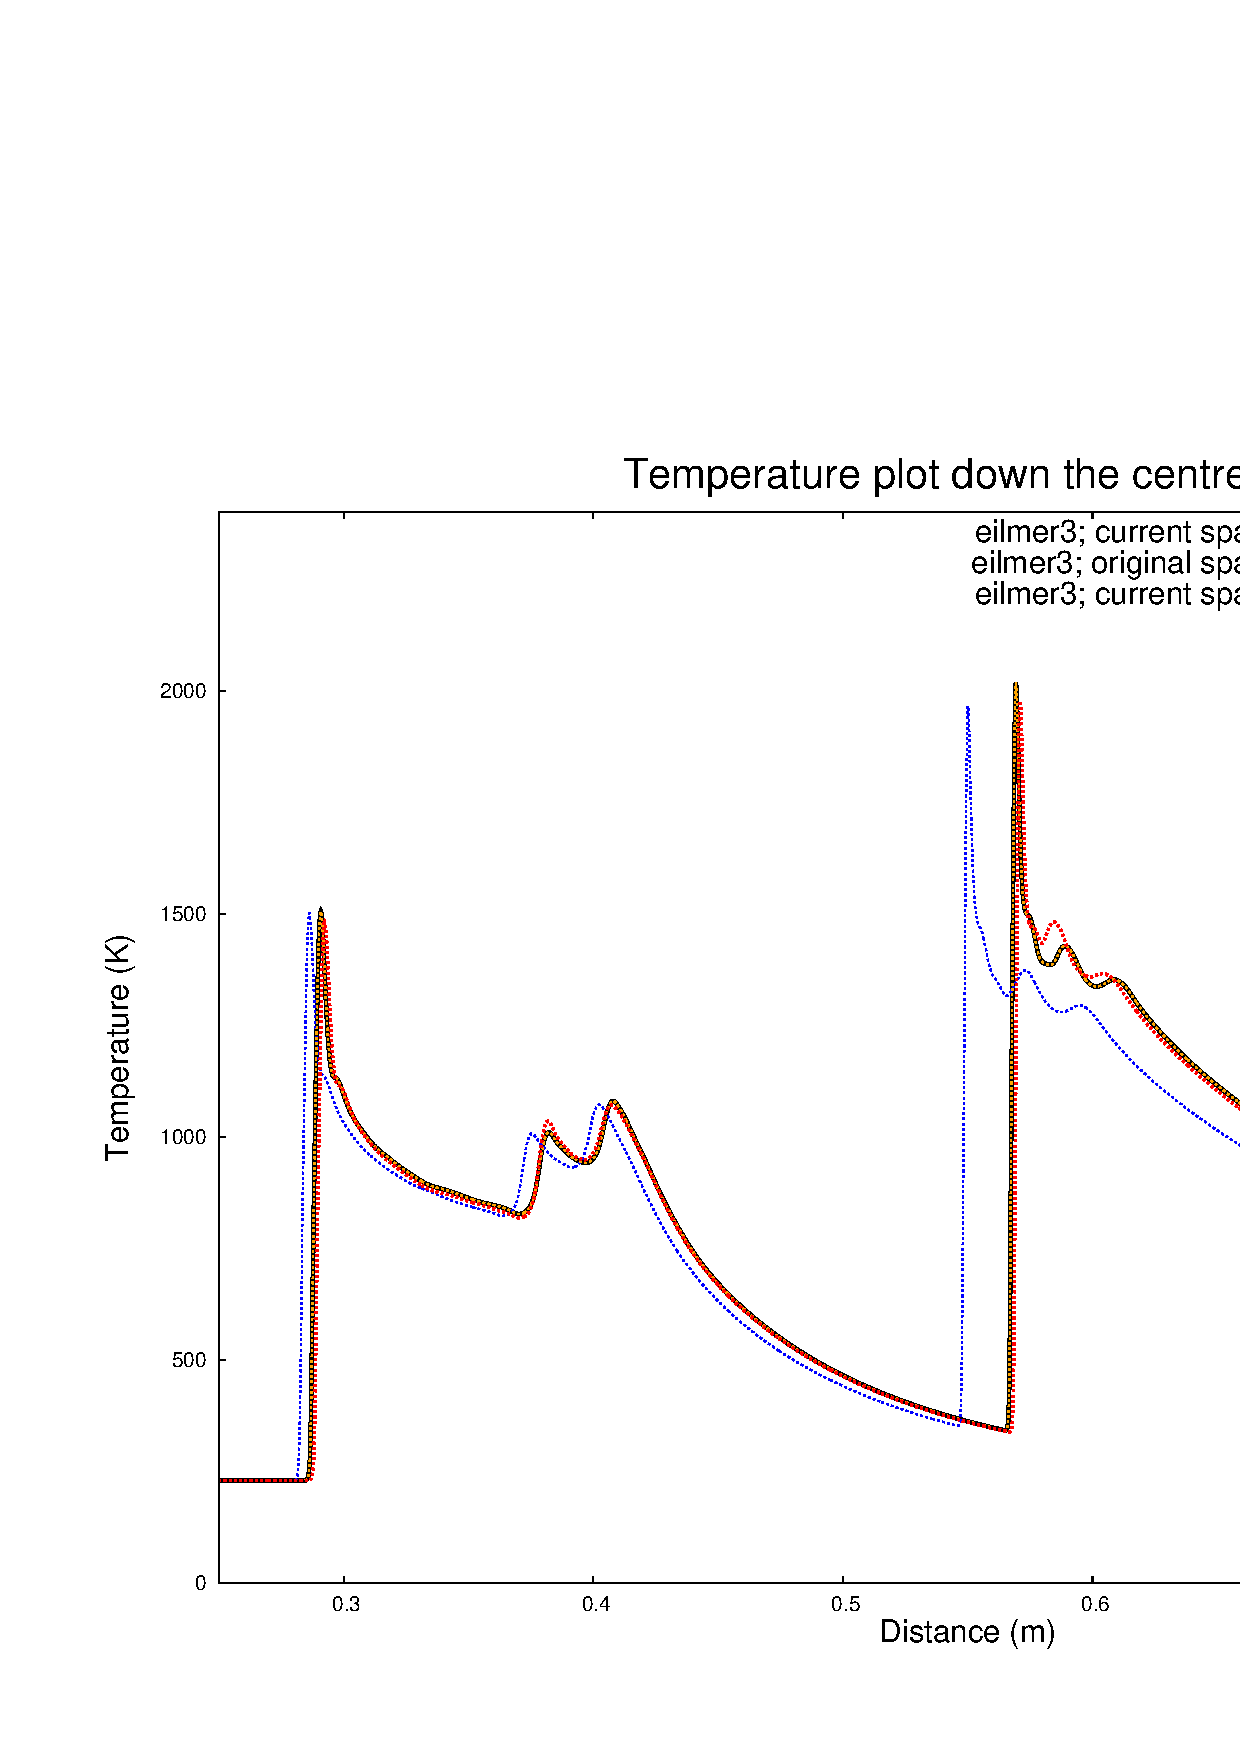
\includegraphics[width=0.9\linewidth]{./chap3-axi-scramjet/T_profile_centreline.pdf}
 % T_profile_centreline.pdf: 792x576 pixel, 72dpi, 27.94x20.32 cm, bb=0 0 792 576
 \caption{Temperature plot down the centreline}
 \label{fig:T_plot}
\end{figure}

The main points to be taken from this plot are the comparisons with the different cases. Firstly, the most noticeable difference is the comparison with the original space marching solver - the spikes have shifted noticeably downstream for the current space marching solver and now matches the results of the time-dependent solver. The previous discrepancy occurred due to the boundary data transfer between the blocks and this shows that the fix that was implemented appears to be working well. Two different computations were completed with the new space marching solver to get an indication of the effect of total simulation time however there is no appreciable difference between 3 and 6 flow lengths. 

Secondly, the other difference that can be seen in the plots occurs at approximately 0.6\,m where the space marched solver and the time resolved solver show slightly different results. This is probably due to a separation occuring in the flow which is not picked up properly by the space marching solver. The final result however is still quite close giving confidence in the use of the space marching solver for preliminary computations.

%--------------------------------------------------------------------

\newpage
\bibliographystyle{unsrt}
\bibliography{./bibtex/pj,./bibtex/computing,./bibtex/gas_dynamic,./bibtex/adm,./bibliography/phd_bibliography}

\newpage
\appendix

% code.tex

\newpage
\section{Code}
\label{code}

The following is the space marching solver code extracted directly out of the \textit{main.cxx} file from eilmer3.

{\scriptsize
\begin{verbatim}
int integrate_blocks_in_sequence( void )
// This procedure integrates the blocks one-at-a-time in sequence.
//
// The idea is to approximate the space-marching approach of sm_3d
// and, hopefully, achieve a significant speed-up over integration
// of the full array of blocks.
//
// It is assumed that we have the restricted case 
// of all the blocks making a single line (west to east) with
// supersonic flow at the west face of block 0 and 
// extrapolate_out on the east face of the final block.
//
// The above assumptions still stand but the code has been modified
// such that the calcluation now does two active blocks at a time.
// The calculation initially does blocks 0 and 1, and then moves over
// one block for the next step calculating blocks 1 and 2 next.
// This process is then repeated for the full calculation

{
    global_data &G = *get_global_data_ptr();
    Block *bdp;
    double time_slice = G.max_time / G.nblock;
    BoundaryCondition *bcp_save;

    // Initially deactivate all blocks
    for ( int jb = 0; jb < G.nblock; ++jb ) {
	bdp = get_block_data_ptr(jb);
	bdp->active = 0;
    }

    cout << "Integrate Block 0 and Block 1" << endl;

    // Start by setting up block 0

    // Activate block 0
    bdp = get_block_data_ptr(0);
    bdp->active = 1;
    // Apply the assumed SupINBC to the west face and propogate across the block
    bdp->bcp[WEST]->apply_inviscid(0.0);
    bdp->propagate_data_west_to_east( G.dimensions );
    bdp->apply( &FV_Cell::encode_conserved, bdp->omegaz, "encode_conserved" );
    // Even though the following call appears redundant at this point,
    // fills in some gas properties such as Prandtl number that is
    // needed for both the cfd_check and the BLomax turbulence model.
    bdp->apply( &FV_Cell::decode_conserved, bdp->omegaz, "decode_conserved" );

    // Now set up block 1

    // Activate block 1
    bdp = get_block_data_ptr(1);
    bdp->active = 1;

    // Save the original east boundary condition and apply the temporary
    // ExtrapolateOutBC for the calculation
    bcp_save = bdp->bcp[EAST];
    bdp->bcp[EAST] = new ExtrapolateOutBC(*bdp, EAST, 0);

    // Read in data from block 0 and propogate across the block
    exchange_shared_boundary_data( 1, COPY_FLOW_STATE);
    bdp->propagate_data_west_to_east( G.dimensions );
    bdp->apply( &FV_Cell::encode_conserved, bdp->omegaz, "encode_conserved" );
    bdp->apply( &FV_Cell::decode_conserved, bdp->omegaz, "decode_conserved" );

    // Integrate just the first two blocks in time, hopefully to steady state.
    set_block_range(0,1);
    integrate_in_time( time_slice );


    // The rest of the blocks.
    for ( int jb = 2; jb < (G.nblock); ++jb ) {
	// jb-2, jb-1, jb
	// jb-2 is the block to be deactivated, jb-1 has been iterated and now
	// becomes the left most block and jb is the new block to be iterated
	cout << "Integrate Block " << jb << endl;
	// Make the block jb-2 inactive.
	bdp = get_block_data_ptr(jb-2);
	bdp->active = 0;

	// block jb-1 - reinstate the previous boundary condition on east face
	// but leave the block active
	bdp = get_block_data_ptr(jb-1);
	delete bdp->bcp[EAST];
	bdp->bcp[EAST] = bcp_save;

	// Set up new block jb to be integrated
	bdp = get_block_data_ptr(jb);
	bdp->active = 1;

	if ( jb < G.nblock-1 ) {
	    // Cut off the east boundary of the current block 
	    // from the downstream blocks if there are any.
	    bcp_save = bdp->bcp[EAST];
	    bdp->bcp[EAST] = new ExtrapolateOutBC(*bdp, EAST, 0);
	}
	// Now copy the starting data into the WEST ghost cells
	// and propagate it across the current block.
	exchange_shared_boundary_data( jb, COPY_FLOW_STATE );
	bdp->propagate_data_west_to_east( G.dimensions );
	bdp->apply( &FV_Cell::encode_conserved, bdp->omegaz, "encode_conserved" );
	bdp->apply( &FV_Cell::decode_conserved, bdp->omegaz, "decode_conserved" );
	// Integrate just the two currently active blocks in time,
	// hopefully to steady state.
	set_block_range(jb-1, jb);
	integrate_in_time( (jb+1)*time_slice );
    }
    // Before leaving, we want all blocks active for output.
    for ( int jb = 0; jb < G.nblock; ++jb ) {
	bdp = get_block_data_ptr(jb);
	bdp->active = 1;
    }
    set_block_range(0, G.nblock - 1);
    return SUCCESS;
} // end integrate_blocks_in_sequence()
}
\end{verbatim}
}

\end{document}
